\documentclass[11pt]{report}
\usepackage[margin=1in]{geometry}
\usepackage{array}
\usepackage{longtable}
\usepackage{titlesec}
\usepackage{graphicx}
\usepackage{parskip}
\usepackage{glossaries}
\usepackage{datetime}
\usepackage{hyperref}
\usepackage{rotating}
\usepackage{float}
\usepackage[toc,page]{appendix}
\usepackage{wrapfig}

\titleformat{\chapter}{\Large\bfseries}{}{0pt}{\huge}
\titlespacing\chapter{0pt}{*1}{*1}
\titlespacing\section{0pt}{*0}{-\parskip}
\titlespacing\subsection{0pt}{*0}{-\parskip}
\titlespacing\paragraph{0pt}{*0}{*3}

\newcolumntype{a}[1]{>{\centering}p{#1}}

\newcommand*{\TitleFont}{
      \usefont{\encodingdefault}{\rmdefault}{b}{n}
      \fontsize{24}{36}
      \selectfont
}
\newcommand*{\SubtitleFont}{
      \usefont{\encodingdefault}{\rmdefault}{}{n}
      \fontsize{12}{12}
      \selectfont
}
\newcommand{\thickline}{\rule{\textwidth}{1.6pt}}
\newcommand{\thinline}{\rule{\textwidth}{0.4pt}}
\newcommand{\novspace}{\vspace*{-\baselineskip}\vspace*{4pt}}
\renewcommand{\dateseparator}{-}
\let\oldtitle\title
\newcommand{\fulltitle}[2]{\oldtitle{\thickline \\ \novspace \thinline \\ \TitleFont {#1} \thinline \\ \novspace \thickline #2}}
\renewcommand{\title}[1]{\fulltitle{#1}{}}
\newcommand{\titleandsubtitle}[2]{\fulltitle{#1}{\\ \SubtitleFont{#2}}}
\newcommand{\tableoffiguresandtables}{\listoffigures\begingroup\let\clearpage\relax\listoftables\endgroup}
\newcommand{\textrotate}[1]{\begin{turn}{-90}#1\end{turn}}
\newcommand{\signature}[1]{\\Signature: & & Date: & \\ \cline{2-2} \cline{4-4}	& #1 & & YYYY-MM-DD \tabularnewline}
\newcommand{\signatures}{\begin{tabular}{ca{8cm}ca{4cm}c}\signature{Evan Milton}\signature{Josh DeWitt}\signature{Chad Staley}\signature{James Gehringer}\end{tabular}}
\newcommand{\minutesessentials}[8]{\section{Meeting #1}
\begin{tabular}{llc}
	Date & #2 & \\
	Time & #3 & \\
	Location & #4 & \\
	Attendance & Evan Milton & #5 \\
	& Josh DeWitt & #6 \\
	& Chad Staley & #7 \\
	& James Gehringer & #8 \\
\end{tabular}}
\newcommand{\minutesdetails}[2]{\paragraph{Agenda}\begin{enumerate}#1\end{enumerate}\paragraph{Decisions Reached}\begin{enumerate}#2\end{enumerate}}

\hypersetup{
	colorlinks,
	citecolor=black,
	filecolor=black,
	linkcolor=black,
	urlcolor=black
}

\author{
	Josh DeWitt \\
	Computer and Electronics Engineering \\
	University of Nebraska-Lincoln \\
	Computer Engineering, minor in Computer Science \\
	Mathematics
}
\date{\yyyymmdddate\today}

\newacronym{2d}{2-D}{Two-Dimensional}
\newacronym{3d}{3-D}{Three-Dimensional}
\newacronym{aon}{AON}{Activity On Node}
\newacronym{arm}{ARM}{Advanced RISC Machines}
\newacronym{bom}{BOM}{Bill of Materials}
\newacronym{cad}{CAD}{Computer-Aided Design}
\newacronym{ceen}{CEEN}{Computer and Electronics Engineering}
\newacronym{cnc}{CNC}{Computer Numerical Control}
\newacronym{cpu}{CPU}{Central Processing Unit}
\newacronym{dmm}{DMM}{Digital Multi-Meter}
\newacronym{drc}{DRC}{Design Rules Check}
\newacronym{dvi}{DVI}{Digital Visual Interface}
\newacronym{eco}{ECO}{Engineering Change Order}
\newacronym{ecr}{ECR}{Engineering Change Request}
\newacronym{emi}{EMI}{Electromagnetic Interference}
\newacronym{fmeca}{FMECA}{Failure Mode, Effects, and Criticality Analysis}
\newacronym{gpio}{GPIO}{General Purpose Input/Output}
\newacronym{ieee}{IEEE}{Institute of Electrical and Electronics Engineers}
\newacronym{jtag}{JTAG}{Joint Test Action Group}
\newacronym{led}{LED}{Light Emitting Diode}
\newacronym{lrc}{LRC}{Linear Responsibility Chart}
\newacronym{mpe}{MPE}{Maximum Permissible Exposure}
\newacronym{mttf}{MTTF}{Mean Time to Failure}
\newacronym{nesc}{NESC}{National Electrical Safety Code}
\newacronym{pcb}{PCB}{Printed Circuit Board}
\newacronym{pi}{Pi}{Raspberry Pi}
\newacronym{pcsc}{PCSC}{Project Common Success Criteria}
\newacronym{pssc}{PSSC}{Project Specific Success Criteria}
\newacronym{tcpip}{TCP/IP}{Transmission Control Protocol/Internet Protocol}
\newacronym{rf}{RF}{Radio Frequency}
\newacronym{sar}{SAR}{Specific Absorption Rate}
\newacronym{smt}{SMT}{Surface Mount Technology}
\newacronym{ti}{TI}{Texas Instruments}
\newacronym{wbs}{WBS}{Work Breakdown Structure}
\newacronym{xp}{XP}{Extreme Programming}

\titleandsubtitle{CNC Interface \\ Reliability and Safety Analysis}{Professional Homework Three}

\begin{document}
\maketitle

\chapter{Reliability and Safety Analysis}

\section{Introduction}
The \gls{cnc} Interface must perform its functions of communicating with the user and a \gls{cnc} accurately and avoid all risks wherever possible to maintain customer satisfaction.
The aim at hobbyists instead of industrial design allows for a less reliable device, as hobbyists enjoy debugging and fixing devices, however the system will not have any unnecessary reliability flaws.
This report contains reliability analysis, safety analysis, and \gls{fmeca} and includes action items to improve the overall reliability of the \gls{cnc} Interface.
The most critical issues in this design involve the inability to immediately halt the \gls{cnc} at the user's request, as these moving components can harm people and property and require safeguards to mitigate risk. 

\section{Reliability Analysis}
The components determined most likely to fail were analyzed for reliability to determine an expected \gls{mttf} for the entire system.
All components chosen are critical and can be considered a series system, so the overall reliability is $R_s(t)=\prod_{i=1}^4R_i(t)$.
This gives an overall failure rate of $\lambda_s=\sum_{i=1}^n\lambda_i$ and a $\gls{mttf}_s=\frac{1}{\lambda_s}$.
Calculation of individual $\lambda$ values was performed based on the Reliability Prediction of Electronic Equipment handbook, MIL-HDBK-217F\cite{mil217f}.

\subsection{Common Parameters}
All devices chosen were best described by the microcircuit model, so several common parameters were found and are shown in table ~\ref{tab:commonparameters} to avoid unnecessary repetition.
\begin{table}[h]
\caption{Common Parameters \gls{mttf} Summary}
\label{tab:commonparameters}
\centering
\begin{tabular}{|>{\centering}m{1.7cm}|>{\centering}m{3.5cm}|>{\centering}m{1cm}|m{9cm}|}
\hline
	Parameter Name & Description & Value & Comments \\ \hline
	$\pi_E$ & Environment Factor & 2.0 & From table in section 5.10\cite{mil217f} given fixed ground environment, that is, moderately controlled environment, not laboratory setting \\ \hline
	$\pi_Q$ & Quality Factors & 2.0 & From table in section 5.10\cite{mil217f} given commercial-grade device \\ \hline
	$\pi_L$ & Learning Factor & 1.0 & From table in section 5.10\cite{mil217f} given production run of over two years \\ \hline
\end{tabular}
\end{table}

\subsection{TMS320F28027 Texas Instruments Microcontroller}
For a microcontroller, the failure rate is $\lambda_p=(C_1\pi_T+C_2\pi_E)\pi_Q\pi_L$ failures$/10^6=796.72*10^{-3}$ failures$/10^6$ hours based on section 5.1\cite{mil217f} using the parameters chosen in tables ~\ref{tab:commonparameters} and ~\ref{tab:tms320f28027parameters}.
This gives a \gls{mttf} of $\frac{1}{\lambda_p}=\frac{10^6}{796.72*10^{-3}}=1.255*10^6$ hours $=143$ years for this component.
\begin{table}[h]
\caption{TMS320F28027 \gls{mttf} Summary}
\label{tab:tms320f28027parameters}
\centering
\begin{tabular}{|>{\centering}m{1.7cm}|>{\centering}m{3.5cm}|>{\centering}m{1cm}|m{9cm}|}
\hline
	Parameter Name & Description & Value & Comments \\ \hline
	$C_1$ & Die Complexity Failure Rate & .56 & From table in section 5.1\cite{mil217f} given 32-bit RISC MOS microcontroller \\ \hline
	$\pi_T$ & Temperature Factor & .646 & $0.1*exp\left(\frac{-E_a}{8.617*10^{-5}}\left(\frac{1}{T_J+273}-\frac{1}{298}\right)\right)$ from section 5.8\cite{mil217f} \\ \hline
	$E_a$ & Effective Activation Energy & .42 & From table in section 5.8\cite{mil217f} given MOS device and $T_J$ \\ \hline
	$T_J$ & Worst Case Junction Temperature & 63.379 & $T_C+\theta_{JC}P$ from section 5.11\cite{mil217f} \\ \hline
	$T_C$ & Case Temperature & 60 & From the \gls{pssc} \\ \hline
	$\theta_{JC}$ & Junction to Case Thermal Resistance & 12.8 & From the datasheet\cite{picollo} \\ \hline
	$P$ & Device Power Dissipation & .264 & From the datasheet\cite{picollo} \\ \hline
	$C_2$ & Package Failure Rate & .0183 & From table in section 5.9\cite{mil217f} given hermetic \gls{smt} device with 48 pins, linear approximation since values are only given for 40 and 64 pins \\ \hline
\end{tabular}
\end{table}

\subsection{OKI-78SR Series 5V Switching Regulator}
For a monolithic MOS device, the failure rate is $\lambda_p=(C_1\pi_T+C_2\pi_E)\pi_Q\pi_L$ failures$/10^6=771*10^{-3}$ failures$/10^6$ hours based on section 5.1\cite{mil217f} using the parameters chosen in tables ~\ref{tab:commonparameters} and ~\ref{tab:oki78srparameters}.
This gives a \gls{mttf} of $\frac{1}{\lambda_p}=\frac{10^6}{771*10^{-3}}=1.297*10^6$ hours $=148$ years for this component.
\begin{table}[h]
\caption{OKI-78SR \gls{mttf} Summary}
\label{tab:oki78srparameters}
\centering
\begin{tabular}{|>{\centering}m{1.7cm}|>{\centering}m{3.5cm}|>{\centering}m{1cm}|m{9cm}|}
\hline
	Parameter Name & Description & Value & Comments \\ \hline
	$C_1$ & Die Complexity Failure Rate & .020 & 101 to 1000 transistor MOS digital device from section 5.1\cite{mil217f} and the datasheet\cite{oki78sr} \\ \hline
	$\pi_T$ & Temperature Factor & 19.18 & $0.1*exp\left(\frac{-E_a}{8.617*10^{-5}}\left(\frac{1}{T_J+273}-\frac{1}{298}\right)\right)$ from section 5.8\cite{mil217f} \\ \hline
	$E_a$ & Effective Activation Energy & .84 & From table in section 5.8\cite{mil217f} given a MOS device and $T_J$  \\ \hline
	$T_J$ & Worst Case Junction Temperature & 82.05 & $T_C+\theta_{JC}P$ from section 5.11\cite{mil217f} \\ \hline
	$T_C$ & Case Temperature & 70 & Assuming a $10^{\circ}C$ temperature increase from the \gls{cpu} temperature specified in the \gls{pssc} \\ \hline
	$\theta_{JC}$ & Junction to Case Thermal Resistance & 13 & From the datasheet \\ \hline
	$P$ & Device Power Dissipation & .927 & Output voltage of 5V, maximum load current of 1.5A with a minimum efficiency of 89\% from the datasheet\cite{oki78sr} \\ \hline
	$C_2$ & Package Failure Rate & .00092 & From table in section 5.9\cite{mil217f} given hermetic package with 3 pins \\ \hline
\end{tabular}
\end{table}

\subsection{LM1117 Texas Instruments Linear Regulator}
For a monolithic bipolar device, the failure rate is $\lambda_p=(C_1\pi_T+C_2\pi_E)\pi_Q\pi_L$ failures$/10^6=71.87$ failures$/10^6$ hours based on section 5.1\cite{mil217f} using the parameters chosen in tables ~\ref{tab:commonparameters} and ~\ref{tab:lm1117parameters}.
This gives a \gls{mttf} of $\frac{1}{\lambda_p}=\frac{10^6}{71.87}=13.914*10^3$ hours $=1.587$ years for this component.
\begin{table}[h]
\caption{LM1117 \gls{mttf} Summary}
\label{tab:lm1117parameters}
\centering
\begin{tabular}{|>{\centering}m{1.7cm}|>{\centering}m{3.5cm}|>{\centering}m{1cm}|m{9cm}|}
\hline
	Parameter Name & Description & Value & Comments \\ \hline
	$C_1$ & Die Complexity Failure Rate & .010 & 1 to 100 transistor bipolar linear device from section 5.1\cite{mil217f} and the datasheet\cite{lm1117}, assuming 30 transistors per op amp and 5 transistors per current source \\ \hline
	$\pi_T$ & Temperature Factor & 3593 & $0.1*exp\left(\frac{-E_a}{8.617*10^{-5}}\left(\frac{1}{T_J+273}-\frac{1}{298}\right)\right)$ from section 5.8\cite{mil217f} \\ \hline
	$E_a$ & Effective Activation Energy & 2.0 & From table in section 5.8\cite{mil217f} given a abipolar device and $T_J$  \\ \hline
	$T_J$ & Worst Case Junction Temperature & 71.38 & $T_C+\theta_{JC}P$ from section 5.11\cite{mil217f} \\ \hline
	$T_C$ & Case Temperature & 65 & Assuming a $5^{\circ}C$ temperature increase from the \gls{cpu} temperature specified in the \gls{pssc} \\ \hline
	$\theta_{JC}$ & Junction to Case Thermal Resistance & 15 & From the datasheet\cite{lm1117} \\ \hline
	$P$ & Device Power Dissipation & .425 & Maximum input voltage of 5V, output voltage of 3.3V, maximum current of 250mA \\ \hline
	$C_2$ & Package Failure Rate & .0013 & From table in section 5.9\cite{mil217f} given hermetic package with 4 pins \\ \hline
\end{tabular}
\end{table}

\subsection{Reliability Analysis Results}
With the three components analyzed, $\lambda_s=796.72*10^{-3}+771*10^{-3}+71.87=73.438$ failures$/10^6$ years, and a \gls{mttf} of $\frac{10^6}{73.438}=13617$ hours $=1.55$ years for the system.
Because the system is aimed at hobbyists, the system need not last for 20 years, but an overall \gls{mttf} of 1.55 years is inadequate.
Initially the 3.3V linear regulator was used for price and simplicity, but it is clearly a liability in the system and should be replaced with a switching regulator like the 5V regulator.
This switching regulator would have a $\lambda$ value less than the 5V regulator component because it would be at a lower temperature and consume less power, giving an overall \gls{mttf} of at least 48.78 years.

The most notable improvement in reliability came from the \gls{pssc} stating a maximum \gls{cpu} temperature of $60^{\circ}C$, which reduced the temperature coefficients in the system in the worst case analysis.
The system will not normally be at $60^{\circ}C$, only in extreme cases.
However, the system would be adequately reliable for hobbyists even if operating at such high temperatures continuously, so long as the linear 3.3V regulator is replaced with a switching regulator.

\section{Safety Analysis}
\gls{ieee} standards were used to guide the safety analysis to understand the risks posed by the \gls{cnc} Interface project.
Safety Analysis Results were based on the analysis of \gls{ieee} standard C95.1\cite{ieeec951}, \gls{ieee} \gls{nesc}\cite{ieeenesc}, and the moving components that will be attached to the system by the end user. 

\subsection{IEEE C95.1 Radio Frequency Analysis}
\gls{ieee} Standard C95.1\cite{ieeec951} uses the \gls{sar} of the human body relating to radio frequencies of 3kHz to 300GHz, which applies to the wireless component of the project.
The project has an \gls{rf} communication component of standard 802.11b/g/n WiFi via a miniature WiFi USB Module, operating in the 2.4GHz range.
The system may have \gls{rf} noise generated by digital switching components, however their power in the 3kHz to 300GHz range will be orders of magnitude less than the WiFi, so they will be ignored for this analysis.
The system is aimed at hobbyists, so the end user will have an uncontrolled environment, meaning that the \gls{mpe} is $10\frac{W}{m^2}$ according to Table 9 in C95.1 chapter 4\cite{ieeec951}.

The WiFi module has a maximum \gls{rf} output power of $17dBm$, which can be re-written as $1mW*10^{\frac{17}{10}}=50.11mW$.
The volume of a sphere is given by $\frac{4}{3}\pi r^2$, so solving the following equation will give the safe radius that a person could regularly be by the device: $\frac{50.11mW}{\frac{4}{3}\pi r^2}=10\frac{W}{m^2}$.
Simple algebra produces a safe distance of $6.13cm$ from the WiFi module, which is a reasonable distance seeing that this device will not be touched by the consumer, only controlled remotely on a regular basis. 
If the user wishes to move the module, they should issue the shutdown command remotely, which powers down the WiFi module, then disconnect the power and move the device to the new desired location.

\subsection{National Electrical Safety Code Analysis}
\gls{ieee}'s \gls{nesc}\cite{ieeenesc} discusses the safety of installing, operating, and maintenance of electric power for all types of building wiring, including residential.
The main safety concern regarding the \gls{nesc} for the \gls{cnc} Interface is the connection between wall power and the system that the user purchases separate of the system.
Since this select cannot be directly controlled, the system will be shipped with guidelines on picking a safe power supply for use with the system.
Because the system will be connecting to a power supply of up to 36V, the system uses an industry-standard connection jack that does not expose the voltage line to the user.
Additionally, all packaging in the system will be made of non-conductive materials, and any exposed metal components will be grounded to avoid the risk of electrical shock\cite{ieeenesc}.

\subsection{Moving Parts Analysis}
The \gls{cnc} Interface does not include the actual motor or work equipment, so the project cannot enforce that the user select a safe work environment for their \gls{cnc}.
The system will be shipped with a large emergency stop button that will stop all motors immediately when pressed.
Software, to be run whenever the system is moved, will be available that prompts the user to press the emergency button and verify that the emergency stop signal was received.
To mitigate the risk of user selection of the work area, the system will be shipped with guidelines on creating a safe work environment for their \gls{cnc}.
These guidelines will include recommendations to have the ability to enclose the work area to avoid physical access to the work area while running the system.
A physical barrier would also help protect against release of parts from the work area during any type of milling procedure.

\subsection{Safety Analysis Results}
The analysis has created the following Safety Requirements that the system must abide by:
\begin{itemize}
	\item Include documentation on safe operating practices for running the \gls{cnc} Interface.
	\item Include documentation on \gls{rf} emissions from the \gls{cnc} Interface.
	\item Include guidelines for selecting an appropriate power supply to use with the \gls{cnc} Interface.
	\item Include safety recommendations when creating a work area to connect to the \gls{cnc} Interface.
	\item Include an emergency stop button that can be placed near the work area for easy access.
	\item Include a system test that ensures that the emergency stop button is connected and works correctly.
\end{itemize}

\section{Failure Mode, Effects, and Criticality Analysis}
The first step for \gls{fmeca} analysis is to break down the schematic into functional blocks. 
See Appendix~\ref{chap:schematic-breakdown} for the detailed contents of each of the four main functional blocks of the circuit.
Figure~\ref{fig:power-block} depicts the voltage regulation circuitry for the system.
Figure~\ref{fig:connectors-block} depicts the off-board data connectors to the \gls{pi} and the the General Purpose Outputs described in the \gls{pssc}.
Figure~\ref{fig:uc-block} depicts the main \gls{ti} microcontroller on the control board.
Figure~\ref{fig:crystal-block} depicts the crystal used to generate the system clock.

For this analysis, only one of the criticality levels, Catastrophic is retained from the Standard Practice for System Safety\cite{mil882d}.
The reason for this is that life-threatening personal injury is still as important, but all other components of a hobbyist's \gls{cnc}, including motors and frame, will not be valued over \$2000.
Analysis of the possible failures modes of each block, effects, criticality, and suggested actions are shown in table~\ref{tab:fmeca}.

\begin{table}[h]
\caption{Criticality Severity Categories}
\label{tab:criticality}
\centering
\begin{tabular}{|>{\centering}m{2cm}|>{\centering}m{2cm}|>{\centering}m{2cm}|m{9cm}|}
\hline
	Criticality Name & Max $\lambda$ & Minimum \gls{mttf} (y) & Criteria \\ \hline
	Catastrophic & $10^-9$ & 114,080 & Could result in death, permanent total disability, or irreversible severe environmental damage that violates law or regulation, or loss greater than \$2000. \\ \hline
	Critical & $5.70*10^{-6}$ & 20 & Entire \gls{cnc} Interface requires replacement or loss greater than \$100 but less than \$2000. \\ \hline
	Marginal & $1.14*10^{-5}$ & 10 & Soldered component in system requires replacement or loss greater than \$20 but less than \$100. \\ \hline
	Negligible & $1.14*10^{-4}$ & 1 & Non-soldered component requires replacement or loss less than \$20. \\ \hline
\end{tabular}
\end{table}

\section{Summary}
This report thoroughly analyzed the reliability, safety, and criticality of failures in the \gls{cnc} interface and has created several action items to improve the system.
Reliability analysis discourages the user of a linear 3.3V regulator at high temperatures, so the design will be changed to include a switching 3.3V regulator.
Safety analysis deemed that the largest risks lie with the end user setting up their own \gls{cnc} work area, so the system will ship with safety instructions and guidelines to avoid any personal or equipment loss.
\gls{fmeca} analysis showed that the system should be shipped with instructions on how to replace the most likely to fail components, including automating firmware upgrades to ensure the bugs in software are resolved as quickly as possible.
\gls{fmeca} analysis also showed that use of the \gls{ti} TMS320F28027 microcontroller's bootloader for firmware upgrades would allow the system to remain untouched to perform software upgrades, decreasing risk during disassembly for programming with \gls{jtag}.
Several system tests were created to increase safety and reliability, including system tests for the emergency stop to be run whenever the system is moved and tests of the \gls{ti} microcontroller's crystal accuracy using UTC fetched over from the Internet.

\begin{appendices}
	\chapter{Schematic Functional Blocks}
\label{chap:schematic-breakdown}

\begin{figure}[h]
\centering
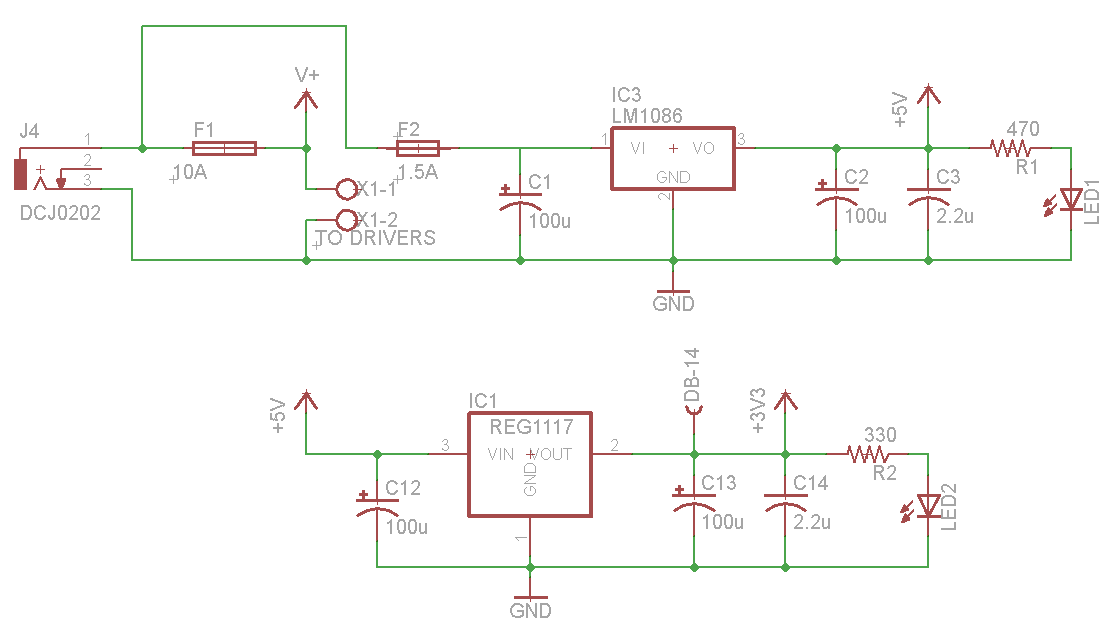
\includegraphics[width=0.6\textwidth]{functional-breakdown-power.png}
\caption{Power Regulation Block}
\label{fig:power-block}
\end{figure}


\begin{figure}[h]
\centering
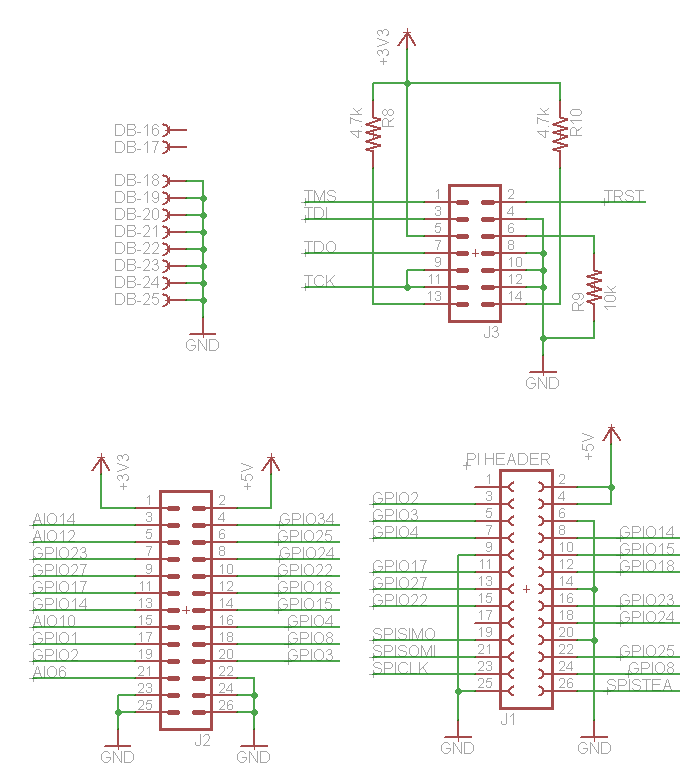
\includegraphics[width=0.5\textwidth]{functional-breakdown-connectors.png}
\caption{Off-Board Connectors Block}
\label{fig:connectors-block}
\end{figure}

\begin{figure}[h]
\centering
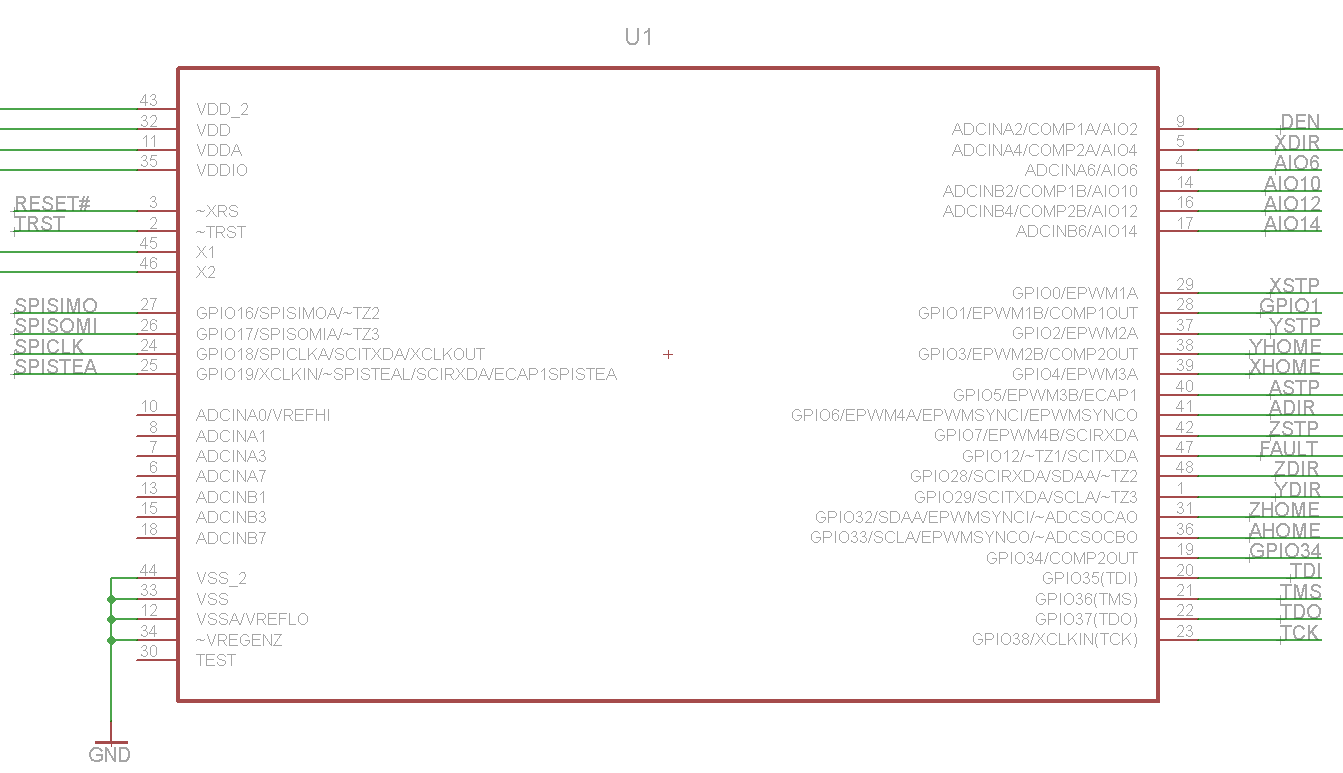
\includegraphics[width=\textwidth]{functional-breakdown-uc.png}
\caption{Microcontroller Block}
\label{fig:uc-block}
\end{figure}

\begin{figure}[h]
\centering
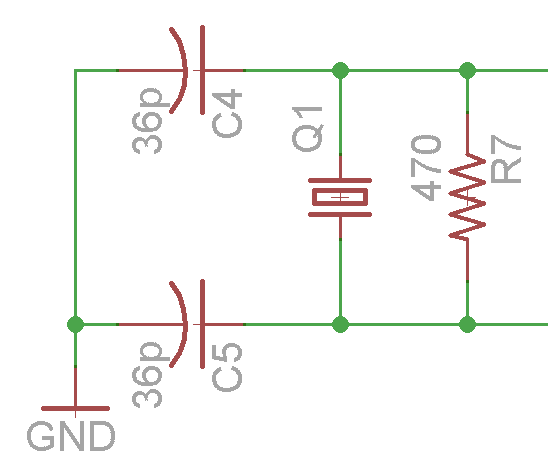
\includegraphics[width=0.5\textwidth]{functional-breakdown-crystal.png}
\caption{Crystal Block}
\label{fig:crystal-block}
\end{figure}


	\chapter{Failure Mode, Effects, and Criticality Analysis}

\begin{table}[h]
\caption{\gls{fmeca} Analysis}
\label{tab:fmeca}
\centering
{\footnotesize
\tabcolsep=0.1cm
\begin{tabular}{|m{2cm}|m{2cm}|m{2cm}|m{3cm}|m{1.5cm}|m{5cm}|}
\hline
	Functional Block & Failure Mode & Failure Cause & Effects & Criticality & Suggested Action \\ \hline
	Power Regulation & 5V rail voltage $>$5V & 5V regulator internal short & Destruction of 3.3V regulator and all microelectronics, including \gls{pi} & Critical & Choose a reliable 5V regulator, include over-voltage protection circuit. \\ \hline
	Power Regulation & 5V rail voltage $<$5V & 5V regulator internal open circuit & No microcontroller on system starts & Marginal & include instructions on replacing the 5V regulator \\ \hline
	Power Regulation & 3.3V rail voltage $>$3.3V & 3.3V regulator internal short & Destruction of all microelectronics on control board & Marginal & Choose a reliable 3.3V regulator, include over-voltage protection circuit \\ \hline
	Power Regulation & 3.3V rail voltage $<$3.3V & 3.3V regulator internal open circuit & Control board microcontroller does not start, \gls{pi} cannot connect to microcontroller & Marginal & Choose a reliable 3.3V regulator, include instructions on replacing the 3.3V regulator \\ \hline
	Off-Board Connectors & Poor electrical connection & Worn out connectors & Poor inter-system communication & Marginal & Design system so that disconnecting and reconnecting of connectors is not frequently required, include instructions on replacing the connectors \\ \hline
	$\mu$Controller & Incorrect control pulses & Bug in code & \gls{cnc} accuracy less than expected & Negligible & Make firmware upgrades possible in-system through bootloader \\ \hline
	Csrystal & No oscillation & Electrical or mechanical shock to crystal & Control board microcontroller does not start & Marginal & Include handling and electrical shock prevention instructions \\ \hline
\end{tabular}
}
\end{table}
	\begin{thebibliography}{9}
\bibitem{mil217f}
	\textit{Reliability Prediction of Electronic Equipment} (MIL-HDBK-217F), 5th ed.,
	Dept. of Defense, Washington, DC,
	1991, pp. 5-1 - 5-24.
\bibitem{picollo}
	\textit{TMS320F2802x, TMS320F2802xx (Piccolo) MCUs},
	\gls{ti}, Dallas, TX,
	2013, pp. 81, 123.
\bibitem{oki78sr}
	\textit{OKI-78SR Series Fixed Output 1.5 Amp SIP DC/DC Converters},
	Murata Power Solutions, Mansfield, MA,
	2013, pp. 1-3.
\bibitem{lm1117}
	\textit{LM1117-N/LM1171 800mA Low-Dropout Linear Regulator},
	\gls{ti}, Dallas, TX,
	2013, pp. 2, 5.
\bibitem{ieeec951}
	\textit{\gls{ieee} Standard for Safety Levels with Respect to Human Exposure to Radio Frequency Electromagnetic Fields, 3kHz to 300GHz} (\gls{ieee} Std C95.1), 2nd ed.,
	\gls{ieee}, New York, NY,
	2005, pp. 20-25.
\bibitem{ieeenesc}
	\textit{National Electrical Safety Code},
	\gls{ieee}, New York, NY,
	2007, pp 17-20, 32-57.
\bibitem{mil882d}
	\textit{Standard Practice for System Safety} (MIL-STD-882D), 4th ed.,
	Dept. of Defense, Washington, DC,
	2000, pp. 18-20.
\bibitem{emicrystal}
	\textit{EMI-Induced Failures in Crystal Oscillators},
	\gls{ieee} Transactions, vol. 33, no. 4, New York, NY,
	1991, pp. 334-341.
\end{thebibliography}
\end{appendices}
\end{document}
